\chapter{Các đa tuyến mômen động lượng, chuyển động xuyên tâm và thang dao động tử}

\section{Sự phụ thuộc góc của hàm sóng}

Một hạt trong trường lực tâm có một tọa độ xuyên tâm và hai tọa độ góc. Trong cơ học cổ điển,
\begin{equation}
\mathbf L=\mathbf r\times\mathbf p
\end{equation}
được bảo toàn như một vectơ. Hướng của vectơ này xác định mặt phẳng quỹ đạo, dù quỹ đạo không nhất thiết là đường tròn.

Trong cơ học lượng tử, hạt được mô tả bởi
\begin{equation}
\Psi=\Psi(r,\theta,\phi),
\end{equation}
và mômen động lượng liên quan đến sự phụ thuộc của hàm sóng này vào các góc.

Trong hai chiều, chỉ có một thành phần mômen động lượng, là toán tử sinh các phép quay quanh trục vuông góc với mặt phẳng:
\begin{equation}
L_z=-i\hbar\frac{\partial}{\partial\theta}.
\end{equation}
Hàm riêng có trị riêng \(\hbar\ell\) thỏa mãn
\begin{equation}
-i\hbar\frac{\partial}{\partial\theta}\psi(r,\theta)
=\hbar\ell\,\psi(r,\theta).
\end{equation}
Trong phương trình này, tọa độ \(r\) chỉ đóng vai trò tham số. Nghiệm có dạng
\begin{equation}
\psi(r,\theta)=\chi(r)e^{i\ell\theta}.
\end{equation}
Với hàm sóng quỹ đạo thông thường, đơn trị, khi trở lại cùng một điểm sau \(\theta\to\theta+2\pi\) thì \(\ell\) phải là một số nguyên. Thừa số xuyên tâm \(\chi(r)\) có thể ảnh hưởng đến năng lượng, nhưng không ảnh hưởng đến trị riêng mômen động lượng này.

Tương tự trong ba chiều, sự phụ thuộc xuyên tâm tách khỏi các hàm trên mặt cầu:
\begin{equation}
\Psi(r,\theta,\phi)=R(r)Y_{\ell m}(\theta,\phi).
\end{equation}
Các hàm \(Y_{\ell m}\) là các điều hòa cầu. Ở đây ta không cần đến công thức tường minh của chúng. Phép quay tác động lên thừa số góc, còn hàm xuyên tâm được giữ nguyên.

\section{Các đa tuyến mômen động lượng hữu hạn}

Các thành phần của mômen động lượng thỏa mãn
\begin{equation}
\begin{aligned}
[L_x,L_y]&=i\hbar L_z,\\
[L_y,L_z]&=i\hbar L_x,\\
[L_z,L_x]&=i\hbar L_y.
\end{aligned}
\end{equation}
Chọn các trạng thái riêng của \(L_z\),
\begin{equation}
L_z|\ell,m\rangle=\hbar m\,|\ell,m\rangle,
\end{equation}
và định nghĩa
\begin{equation}
L_\pm=L_x\pm iL_y.
\end{equation}
Các hệ thức giao hoán
\begin{equation}
[L_z,L_\pm]=\pm\hbar L_\pm
\end{equation}
suy ra
\begin{align}
L_z\bigl(L_\pm|\ell,m\rangle\bigr)
&=\bigl(L_\pm L_z+[L_z,L_\pm]\bigr)|\ell,m\rangle \\
&=\hbar(m\pm1)L_\pm|\ell,m\rangle.
\end{align}
Vì vậy, \(L_+\) làm tăng \(m\) thêm một đơn vị, còn \(L_-\) làm giảm nó đi một đơn vị, trừ khi vectơ thu được bằng không.

Với một đa tuyến hữu hạn, có trạng thái cao nhất và trạng thái thấp nhất:
\begin{equation}
L_+|\ell,\ell\rangle=0,
\qquad
L_-|\ell,-\ell\rangle=0.
\end{equation}
Các hướng \(+z\) và \(-z\) liên hệ với nhau qua một phép quay, nên phổ hữu hạn đối xứng quanh không. Do đó, các giá trị của nó là
\begin{equation}
m=-\ell,-\ell+1,\ldots,\ell-1,\ell,
\end{equation}
và số trạng thái là
\begin{equation}
2\ell+1.
\end{equation}
Vì các giá trị kề nhau sai khác nhau một đơn vị, hai đầu mút có thể là số nguyên hoặc bán nguyên. Các điều hòa cầu quỹ đạo thông thường hiện thực trường hợp số nguyên; đại số mômen động lượng trừu tượng cũng cho phép các đa tuyến bán nguyên.

\begin{classroomqa}\lecturetimestamp{00:16:12}\audiencequestion{Một đa tuyến mômen động lượng có thể chứa vô hạn trạng thái không?}\lecturerresponse{Có thể xét đến khả năng đó, nhưng ở đây ta không cần dùng đến. Mômen động lượng thường làm tăng năng lượng khi giữ nguyên các đặc điểm khác của trạng thái, nên các trạng thái có mômen động lượng vô hạn không liên quan đến việc khảo sát các trạng thái có năng lượng hữu hạn.}\end{classroomqa}

\section{Giá trị chung của \texorpdfstring{\(L^2\)}{L bình phương}}

Toán tử đo bình phương độ lớn mômen động lượng là
\begin{equation}
L^2=L_x^2+L_y^2+L_z^2.
\end{equation}
Tích có thứ tự của các toán tử bậc thang là
\begin{align}
L_-L_+
&=(L_x-iL_y)(L_x+iL_y) \\
&=L_x^2+L_y^2+i[L_x,L_y] \\
&=L_x^2+L_y^2-\hbar L_z.
\end{align}
Do đó,
\begin{equation}
L^2=L_z^2+\hbar L_z+L_-L_+.
\end{equation}
Áp dụng hệ thức này cho trạng thái cao nhất. Vì \(L_+|\ell,\ell\rangle=0\),
\begin{align}
L^2|\ell,\ell\rangle
&=\left(L_z^2+\hbar L_z+L_-L_+\right)|\ell,\ell\rangle \\
&=\hbar^2\left(\ell^2+\ell\right)|\ell,\ell\rangle,
\end{align}
và do đó
\begin{equation}
L^2|\ell,\ell\rangle
=\hbar^2\ell(\ell+1)|\ell,\ell\rangle.
\end{equation}
Bình phương độ lớn không bằng \(\hbar^2\ell^2\). Số hạng bổ sung xuất hiện do các thành phần mômen động lượng không giao hoán với nhau.

Cùng giá trị này thuộc về mọi trạng thái trong đa tuyến, chứ không chỉ trạng thái cao nhất.

\begin{classroomqa}\lecturetimestamp{00:26:08}\audiencequestion{Bài tập thực sự chứng minh các trạng thái khác có cùng giá trị \(L^2\) như thế nào?}\lecturerresponse{Hãy chứng minh rằng \(L^2\) giao hoán với mọi thành phần mômen động lượng, và do đó giao hoán với \(L_-\). Sau đó đưa \(L^2\) qua \(L_-\): nếu trạng thái cao nhất có trị riêng \(\hbar^2\ell(\ell+1)\), thì trạng thái thấp hơn kế tiếp cũng có cùng trị riêng. Lặp lại lập luận này sẽ truyền giá trị đó dọc theo toàn bộ thang.}\end{classroomqa}

Thật vậy,
\begin{equation}
[L^2,L_i]=0,
\qquad i=x,y,z,
\end{equation}
nên
\begin{equation}
[L^2,L_\pm]=0.
\end{equation}
Chẳng hạn,
\begin{align}
L^2\bigl(L_-|\ell,\ell\rangle\bigr)
&=L_-L^2|\ell,\ell\rangle \\
&=\hbar^2\ell(\ell+1)L_-|\ell,\ell\rangle.
\end{align}
Tiếp tục đi xuống, ta được
\begin{equation}
L^2|\ell,m\rangle
=\hbar^2\ell(\ell+1)|\ell,m\rangle
\end{equation}
cho mọi \(m=-\ell,\ldots,\ell\).

Thứ tự ngược lại cũng cho một phép phân tích tương đương:
\begin{align}
L_+L_-
&=(L_x+iL_y)(L_x-iL_y) \\
&=L_x^2+L_y^2-i[L_x,L_y] \\
&=L_x^2+L_y^2+\hbar L_z,
\end{align}
và do đó
\begin{equation}
L^2=L_z^2-\hbar L_z+L_+L_-.
\end{equation}

\begin{classroomqa}\lecturetimestamp{00:32:05}\audiencequestion{Có thể phân tích \(L_x^2+L_y^2\) theo thứ tự ngược lại, dùng \(L_+L_-\) không?}\lecturerresponse{Có. Dấu của số hạng \(L_z\) bị đảo ngược. Với thứ tự đó, áp dụng hệ thức cho trạng thái thấp nhất, vốn bị triệt tiêu bởi \(L_-\), thay vì trạng thái cao nhất. Ta vẫn thu được cùng trị riêng \(\hbar^2\ell(\ell+1)\).}\end{classroomqa}

Do đó, các điều hòa cầu thỏa mãn
\begin{align}
L^2Y_{\ell m}
&=\hbar^2\ell(\ell+1)Y_{\ell m}, \\
L_zY_{\ell m}
&=\hbar m\,Y_{\ell m}.
\end{align}
Với mỗi giá trị quỹ đạo \(\ell=0,1,2,\ldots\), có \(2\ell+1\) hàm được ký hiệu bằng \(m=-\ell,\ldots,\ell\).

Với thế tâm,
\begin{equation}
[H,L_i]=0.
\end{equation}
Khi đã cố định một trạng thái riêng năng lượng xuyên tâm và \(\ell\), thay đổi \(m\) bằng \(L_\pm\) không làm thay đổi năng lượng. Vì vậy, mỗi trạng thái riêng xuyên tâm như thế tạo thành một đa tuyến từ gồm \(2\ell+1\) trạng thái.

Thang mômen động lượng quỹ đạo nguyên được minh họa bên dưới.\footnote{Sơ đồ được dựng lại từ hình phác họa đa tuyến và các hệ thức toán tử có thể thấy tại \(00{:}35{:}53\) trong video bài giảng.}

\begin{figure}[htbp]\centering
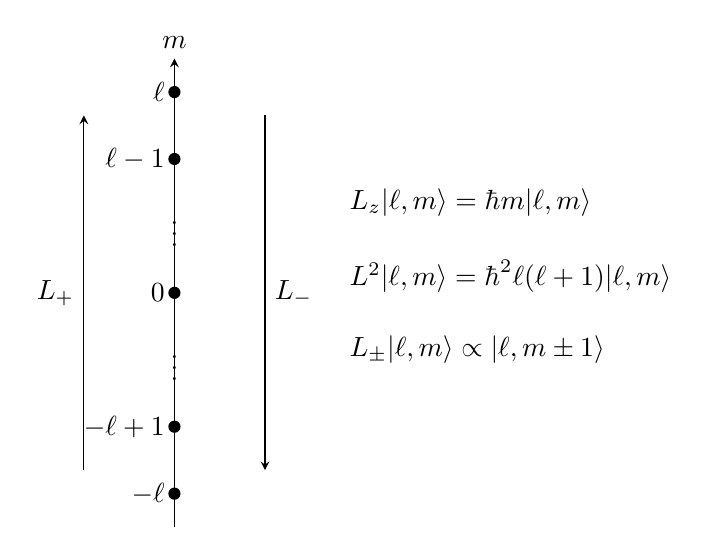
\begin{tikzpicture}[x=1cm,y=0.85cm,>=stealth]
\draw[->] (0,-3.5) -- (0,3.5) node[above] {$m$};

\fill (0,3) circle (2.2pt);
\fill (0,2) circle (2.2pt);
\fill (0,0) circle (2.2pt);
\fill (0,-2) circle (2.2pt);
\fill (0,-3) circle (2.2pt);

\node[left] at (0,3) {$\ell$};
\node[left] at (0,2) {$\ell-1$};
\node[left] at (0,0) {$0$};
\node[left] at (0,-2) {$-\ell+1$};
\node[left] at (0,-3) {$-\ell$};

\node at (0,1) {$\vdots$};
\node at (0,-1) {$\vdots$};

\draw[->] (-1.15,-2.65) -- (-1.15,2.65)
node[midway,left] {$L_+$};
\draw[->] (1.15,2.65) -- (1.15,-2.65)
node[midway,right] {$L_-$};

\node[anchor=west] at (2.1,1.35)
{$L_z|\ell,m\rangle=\hbar m|\ell,m\rangle$};
\node[anchor=west] at (2.1,0.25)
{$L^2|\ell,m\rangle=\hbar^2\ell(\ell+1)|\ell,m\rangle$};
\node[anchor=west] at (2.1,-0.85)
{$L_\pm|\ell,m\rangle\propto|\ell,m\pm1\rangle$};
\end{tikzpicture}\caption{Một đa tuyến mômen động lượng quỹ đạo nguyên. \(L_+\) và \(L_-\) làm thay đổi \(m\) mỗi lần một đơn vị, còn \(L^2\) giữ nguyên giá trị \(\hbar^2\ell(\ell+1)\) trong toàn bộ đa tuyến.}\lectureframe{00:35:53}\end{figure}

\section{Bài toán lực tâm}

Xét
\begin{equation}
H=\frac{\mathbf p^2}{2m}+V(r),
\end{equation}
trong đó \(V\) chỉ phụ thuộc vào khoảng cách đến gốc tọa độ. Đối xứng quay kéo theo sự bảo toàn mômen động lượng. Trong cơ học cổ điển, \(\mathbf L\) có độ lớn và hướng không đổi, nên quỹ đạo luôn nằm trong một mặt phẳng vuông góc với \(\mathbf L\). Quỹ đạo không nhất thiết là đường tròn, thậm chí cũng không nhất thiết là đường kín.

Chọn hệ tọa độ sao cho mặt phẳng quỹ đạo cổ điển là mặt phẳng \(xy\), rồi phân tích động lượng thành các thành phần xuyên tâm và tiếp tuyến:
\begin{equation}
\mathbf p^2=p_r^2+p_\theta^2.
\end{equation}
Vì độ lớn mômen động lượng là
\begin{equation}
L=r p_\theta,
\end{equation}
nên thành phần tiếp tuyến có thể viết là
\begin{equation}
p_\theta^2=\frac{L^2}{r^2}.
\end{equation}
Hamiltonian trở thành
\begin{equation}
H=\frac{p_r^2}{2m}+\frac{L^2}{2mr^2}+V(r).
\end{equation}
Khi \(L\) cố định, đây là bài toán một chiều theo tọa độ xuyên tâm, với thế hiệu dụng
\begin{equation}
V_{\mathrm{eff}}(r)=\frac{L^2}{2mr^2}+V(r).
\end{equation}
Hamiltonian xuyên tâm được trình bày trên bảng bên dưới.\footnote{Khung hình nguồn: \texttt{\detokenize{lecture_03_frame_02.png}}, tại \(00{:}47{:}15\) trong video bài giảng.}

\begin{figure}[htbp]\centering
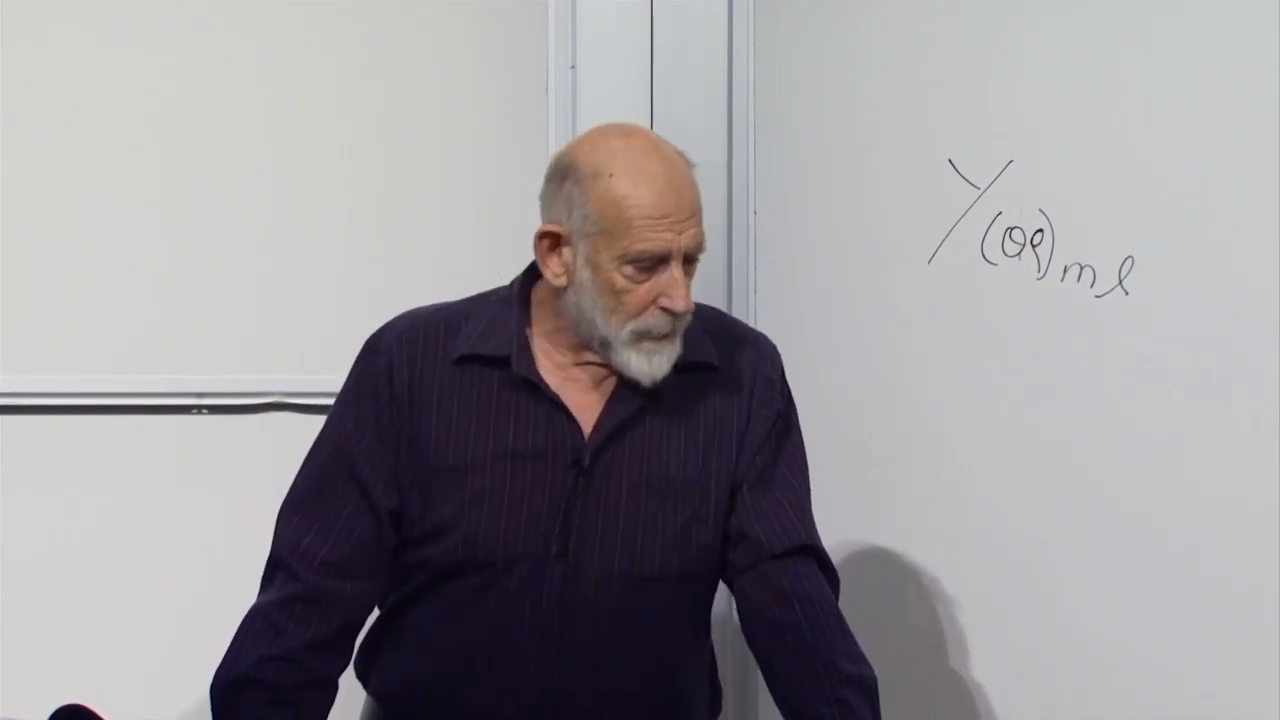
\includegraphics[width=0.9\linewidth]{lecture_03_frame_02.png}\caption{Với mômen động lượng cổ điển cố định, Hamiltonian xuyên tâm gồm động năng xuyên tâm, số hạng ly tâm \(L^2/(2mr^2)\) và thế tâm \(V(r)\).}\lectureframe{00:47:15}\end{figure}

Số hạng \(1/r^2\) là hàng rào ly tâm. Nó tăng lên khi hạt tiến gần gốc tọa độ, nên lực tương ứng hướng ra ngoài. Với các lực hút kiểu Coulomb đang xét, quỹ đạo có \(L\neq0\) sẽ lượn quanh tâm thay vì đi tới tâm. Khi \(L=0\), hàng rào không còn.

Với thế Coulomb hút,
\begin{equation}
V(r)=-\frac{\kappa}{r},
\end{equation}
số hạng ly tâm chiếm ưu thế khi \(r\) nhỏ, còn số hạng Coulomb giảm chậm hơn và chiếm ưu thế khi \(r\) lớn. Khi \(L\neq0\), tổng hai số hạng có một cực tiểu. Chuyển động tại cực tiểu có bán kính không đổi, nên là chuyển động tròn. Chuyển động liên kết với năng lượng cao hơn cực tiểu nhưng thấp hơn ngưỡng thoát dao động giữa bán kính nhỏ nhất và lớn nhất; trong bài toán Coulomb, đó là các dao động xuyên tâm của quỹ đạo elip.

\section{Phương trình xuyên tâm rút gọn}

Trong cơ học lượng tử, phần góc của trạng thái có mômen động lượng quỹ đạo xác định là một điều hòa cầu. Viết trạng thái đã tách biến dưới dạng
\begin{equation}
\Psi_{n_r\ell m}(r,\theta,\phi)
=\frac{u_{n_r\ell}(r)}{r}\,
Y_{\ell m}(\theta,\phi).
\end{equation}
Toán tử góc \(L^2\) có trị riêng
\begin{equation}
L^2Y_{\ell m}
=\hbar^2\ell(\ell+1)Y_{\ell m}.
\end{equation}
Với một cặp \(n_r,\ell\) cố định, viết gọn \(u_{n_r\ell}(r)\) thành \(u(r)\). Phương trình còn lại cho hàm xuyên tâm rút gọn là
\begin{equation}
\begin{aligned}
&-\frac{\hbar^2}{2m}\frac{d^2u}{dr^2}
+\frac{\hbar^2\ell(\ell+1)}{2mr^2}u(r)\\
&\qquad+V(r)u(r)=E_{n_r\ell}\,u(r).
\end{aligned}
\end{equation}

\editorialnote{Phương trình chỉ chứa đạo hàm bậc hai một chiều thuần túy sử dụng hàm xuyên tâm rút gọn \(u=rR\). Vì vậy, \(\psi(r)\) trong phương trình trên bảng của bài giảng tương ứng với \(u(r)\), còn thừa số xuyên tâm thông thường trong \(\Psi=R(r)Y_{\ell m}\) là \(R=u/r\). Quy ước này tránh xem \(-i\hbar\,d/dr\) như một toán tử động lượng xuyên tâm Hermite độc lập trên không gian Hilbert xuyên tâm ba chiều.}

Phương trình xuyên tâm rút gọn được trình bày trên bảng bên dưới.\footnote{Khung hình nguồn: \texttt{\detokenize{lecture_03_frame_03.png}}, tại \(00{:}54{:}32\) trong video bài giảng.}

\begin{figure}[htbp]\centering
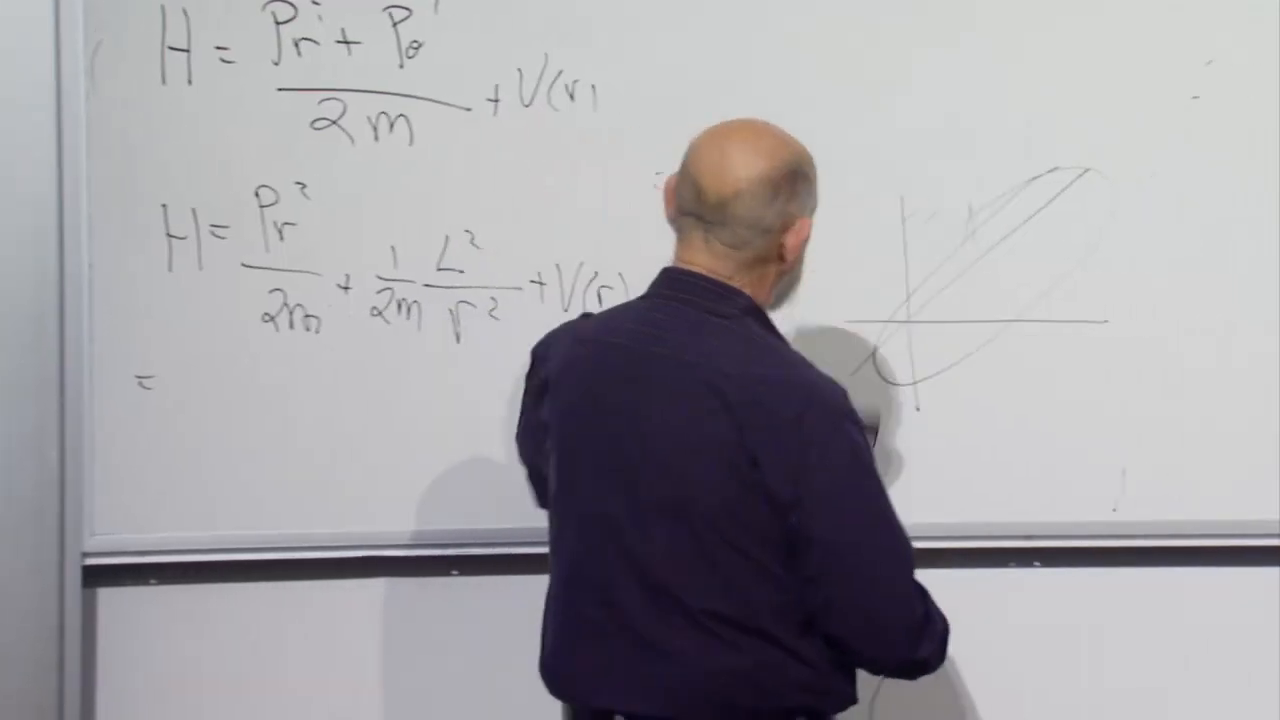
\includegraphics[width=0.9\linewidth]{lecture_03_frame_03.png}\caption{Với \(\ell\) cố định, hàm sóng xuyên tâm rút gọn thỏa mãn phương trình Schr\"odinger một chiều, có số hạng ly tâm tỷ lệ với \(\ell(\ell+1)/r^2\).}\lectureframe{00:54:32}\end{figure}

Cấu trúc góc ba chiều được gói gọn trong tham số \(\ell\). Số lượng tử từ \(m\) không xuất hiện trong phương trình xuyên tâm.

\begin{classroomqa}\lecturetimestamp{00:55:34}\audiencequestion{Với một \(\ell\) cho trước, \(2\ell+1\) trạng thái từ có cùng năng lượng không?}\lecturerresponse{Có, với điều kiện trạng thái riêng xuyên tâm cũng được giữ cố định. Với mỗi \(u_{n_r\ell}\) đã chọn, mọi giá trị \(m=-\ell,\ldots,\ell\) đều có cùng năng lượng vì \(m\) không xuất hiện trong phương trình xuyên tâm. Nói chung, các trạng thái riêng xuyên tâm khác nhau ứng với cùng \(\ell\) có năng lượng khác nhau.}\end{classroomqa}

\begin{classroomqa}\lecturetimestamp{00:56:03}\audiencequestion{Vì sao có thể thay \(L^2\) bằng \(\hbar^2\ell(\ell+1)\), và \(\ell\) liên hệ thế nào với các giá trị được phép của \(m\)?}\lecturerresponse{Số \(\ell\) dùng để ký hiệu một đa tuyến mômen động lượng và là giá trị \(m\) lớn nhất của nó. Mọi trạng thái trong đa tuyến đó đều có cùng trị riêng của \(L^2\), là \(\hbar^2\ell(\ell+1)\), nên ta thay trị riêng ấy vào phương trình xuyên tâm.}\end{classroomqa}

Các nghiệm tường minh bằng hàm đặc biệt không cần thiết cho lập luận hiện tại. Điều quan trọng là cách tổ chức các nghiệm.

\section{Nút xuyên tâm và các mức năng lượng}

Với \(\ell\) cố định, phương trình xuyên tâm rút gọn là một bài toán trị riêng thông thường một chiều. Các trạng thái liên kết được xếp theo số nút bên trong. Trạng thái xuyên tâm thấp nhất không có nút bên trong, trạng thái kế tiếp có một nút, còn trạng thái sau đó có hai nút. Nhiều nút hơn nghĩa là hàm sóng biến thiên nhanh hơn; hàm sóng biến thiên nhanh hơn thì động lượng lớn hơn, do đó động năng cũng lớn hơn.

Mỗi giá trị \(\ell\) xác định một toán tử xuyên tâm khác nhau vì số hạng ly tâm thay đổi theo \(\ell\). Do đó, các \(\ell=0,1,2,\ldots\) tạo thành những tháp mức xuyên tâm riêng biệt. Số hạng ly tâm dương đẩy các mức lên cao hơn khi mômen động lượng tăng. Mỗi trị riêng xuyên tâm ứng với \(\ell\) cố định đều có một đa tuyến từ với số chiều
\begin{equation}
2\ell+1.
\end{equation}
Các mức \(\ell=0\) là đơn tuyến, các mức \(\ell=1\) là tam tuyến, còn các mức \(\ell=2\) là ngũ tuyến. Đây là các độ suy biến do đối xứng quay bảo đảm; một đối xứng bổ sung cũng có thể khiến các trạng thái ứng với những giá trị \(\ell\) khác nhau suy biến cùng mức năng lượng.

Với các thế kiểu nguyên tử thỏa mãn \(V(r)\to0\) khi \(r\) lớn, quy ước chọn ngưỡng thoát là \(E=0\). Các trạng thái năng lượng âm tạo thành phổ liên kết rời rạc. Tại và phía trên \(E=0\), ta gặp phổ liên tục tán xạ. Nhận định này phụ thuộc vào hành vi của thế khi \(r\) lớn, và không áp dụng cho thế tâm giam hãm.

\section{Sự suy biến đặc biệt của thế Coulomb}

Thế Coulomb phi tương đối tính chính xác có thêm một sự trùng khớp giữa các mức năng lượng. Trạng thái xuyên tâm thấp nhất ứng với \(\ell=1\) có cùng năng lượng với trạng thái kích thích thứ nhất ứng với \(\ell=0\). Trạng thái \(\ell=1\) kế tiếp trùng mức với trạng thái kích thích thứ hai ứng với \(\ell=0\), còn trạng thái thấp nhất ứng với \(\ell=2\) cũng cùng mức với chúng. Quy luật này tiếp tục ở các tháp mức xuyên tâm và mômen động lượng cao hơn.

\begin{classroomqa}\lecturetimestamp{01:09:57}\audiencequestion{Sự suy biến Coulomb bổ sung này có cho thấy một đối xứng khác không?}\lecturerresponse{Có. Đây là một đối xứng bổ sung khác thường của thế Coulomb chính xác. Những thay đổi nhỏ của thế sẽ phá vỡ sự trùng khớp này; ta không trình bày cách suy ra nó ở đây.}\end{classroomqa}

Do đó, độ suy biến của các lớp vỏ quỹ đạo là
\begin{equation}
1,\qquad 4,\qquad 9,\qquad 16,\qquad \ldots
\end{equation}
trước khi tính đến spin electron.

\begin{classroomqa}\lecturetimestamp{01:11:46}\audiencequestion{Độ suy biến này mô tả nguyên tử hydro hay chỉ đúng với bài toán Coulomb lý tưởng?}\lecturerresponse{Nguyên tử hydro thỏa mãn kết quả này với độ chính xác rất cao, nhưng không hoàn toàn chính xác. Các hiệu chỉnh tương đối tính và kích thước hữu hạn của hạt nhân làm biến dạng quy luật Coulomb lý tưởng.}\end{classroomqa}

Hạt nhân điểm tạo ra thế \(1/r\) chính xác. Hạt nhân có điện tích phân bố trong một thể tích nhỏ tạo ra thế hơi khác khi electron xuyên vào thể tích đó; ngay cả sai khác nhỏ này cũng làm mất một phần suy biến đặc biệt.

Spin cũng chưa được tính đến. Nếu tính hai trạng thái spin của electron, số trạng thái trong mỗi lớp vỏ tăng gấp đôi, thành
\begin{equation}
2,\qquad 8,\qquad 18,\qquad 32,\qquad \ldots
\end{equation}
trước khi xét đến các độ tách mức bổ sung trong mô tả nguyên tử đầy đủ hơn.

\section{Trở lại phương trình Descartes}

Phương trình ban đầu dẫn đến bài toán xuyên tâm là phương trình Schr\"odinger ba chiều không phụ thuộc thời gian:
\begin{equation}
\begin{aligned}
-\frac{\hbar^2}{2m}\nabla^2\Psi+V(r)\Psi&=E\Psi,\\
\nabla^2&=\frac{\partial^2}{\partial x^2}
+\frac{\partial^2}{\partial y^2}
+\frac{\partial^2}{\partial z^2},\\
r&=\sqrt{x^2+y^2+z^2}.
\end{aligned}
\end{equation}
Chuyển sang tọa độ xuyên tâm và góc, rồi chọn một trạng thái riêng của \(L^2\).
Thay \(L^2\) bằng \(\hbar^2\ell(\ell+1)\) sẽ rút phương trình đạo hàm riêng thành phương trình vi phân thường theo tọa độ xuyên tâm đã nêu ở trên.

\begin{classroomqa}\lecturetimestamp{01:16:42}\audiencequestion{Có thể dùng những sai lệch so với phổ Coulomb lý tưởng để xác định kích thước hạt nhân không?}\lecturerresponse{Không thể chỉ dựa vào phép so sánh đơn giản này. Trước hết phải tính đến các hiệu chỉnh khác lớn hơn nhiều. Ở đây nhắc đến kích thước hạt nhân vì đó là ví dụ trực tiếp cho thấy thế Coulomb của hạt nhân điểm có thể sai khác như thế nào.}\end{classroomqa}

\begin{classroomqa}\lecturetimestamp{01:17:09}\audiencequestion{Khác biệt chính giữa số hạng mômen động lượng cổ điển và lượng tử là gì?}\lecturerresponse{Trong cơ học cổ điển, \(L^2\) là bình phương thông thường của độ lớn một vectơ được bảo toàn. Trong một đa tuyến quỹ đạo lượng tử, trị riêng của nó là \(\hbar^2\ell(\ell+1)\), chứ không đơn giản là \(\hbar^2\ell^2\). Số hạng bổ sung xuất hiện do các thành phần mômen động lượng không giao hoán với nhau.}\end{classroomqa}

\begin{classroomqa}\lecturetimestamp{01:17:58}\audiencequestion{Hàm sóng của trạng thái liên kết có miền hỗ trợ compact không?}\lecturerresponse{Không. Chúng vươn ra xa tâm tùy ý. Với các trạng thái liên kết nguyên tử đang xét, biên độ giảm theo hàm mũ ở khoảng cách lớn, nên xác suất trở nên không đáng kể nhưng không triệt tiêu bên ngoài bất kỳ bán kính hữu hạn nào.}\end{classroomqa}

\begin{classroomqa}\lecturetimestamp{01:18:48}\audiencequestion{Khi \(\ell=0\) làm mất giếng ly tâm, điểm cân bằng ổn định sẽ ra sao?}\lecturerresponse{Không còn cực tiểu do sự cạnh tranh giữa hàng rào ly tâm và lực hút tạo ra. Trong mô hình lý tưởng Coulomb điểm, chuyển động cổ điển hướng về tâm kỳ dị. Trong cơ học lượng tử, trạng thái thấp nhất không thể đồng thời có vị trí xác định chính xác tại tâm và động lượng bằng không, nên hàm sóng thấp nhất có độ trải rộng không gian hữu hạn.}\end{classroomqa}

\editorialnote{Với thế tâm chính quy, quỹ đạo cổ điển có mômen động lượng bằng không có thể tiếp tục đi qua gốc tọa độ. Còn với thế Coulomb điểm lý tưởng, \(r=0\) là một điểm kỳ dị va chạm; muốn tiếp tục quỹ đạo cổ điển thì cần thêm một quy tắc xác định.}

Phép rút gọn cổ điển đặt một quỹ đạo duy nhất vào một mặt phẳng, nhưng không thể áp dụng tương tự cho hàm sóng lượng tử. Một trạng thái quỹ đạo lượng tử trải rộng trong không gian ba chiều. Toán tử góc đầy đủ là \(L^2=L_x^2+L_y^2+L_z^2\), và trị riêng của nó giữ nguyên kết quả ba chiều \(\hbar^2\ell(\ell+1)\).

\begin{classroomqa}\lecturetimestamp{01:21:30}\audiencequestion{Vì sao bài toán lượng tử vẫn là bài toán ba chiều sau khi quỹ đạo cổ điển đã được đặt vào một mặt phẳng?}\lecturerresponse{Chỉ quỹ đạo cổ điển được đặt vào một mặt phẳng cố định bằng cách chọn hệ tọa độ vuông góc với vectơ mômen động lượng bảo toàn của nó. Hàm sóng lượng tử tồn tại trong không gian ba chiều. Các thành phần mômen động lượng còn lại vẫn hiện diện thông qua \(L^2\), đó là lý do phương trình xuyên tâm chứa \(\ell(\ell+1)\) chứ không chỉ chứa bình phương của một thành phần duy nhất.}\end{classroomqa}

\begin{classroomqa}\lecturetimestamp{01:22:54}\audiencequestion{Mọi bài toán lượng tử đều có toán tử nâng và hạ không?}\lecturerresponse{Không. Chúng chỉ xuất hiện trong một số trường hợp đặc biệt thuận lợi. Mômen động lượng là một trường hợp như vậy, và dao động tử điều hòa là một trường hợp khác. Trường hợp dao động tử đặc biệt hữu ích vì chuyển động quanh một cân bằng bền thường gần đúng là dao động điều hòa, kể cả các dao động xuyên tâm nhỏ quanh cực tiểu của thế hiệu dụng.}\end{classroomqa}

Đến đây, ta tạm gác bài toán nguyên tử và chuyển sang dao động tử điều hòa, ví dụ tiếp theo về phổ được xác định bằng các toán tử bậc thang.

\section{Dao động nhỏ và dao động tử điều hòa}

Gần một vị trí cân bằng bền, một độ dời đủ nhỏ thường tạo ra dao động điều hòa. Thế xuyên tâm hiệu dụng khi mômen động lượng khác không là một ví dụ: chuyển động xuyên tâm gần đáy giếng thế gần đúng là dao động điều hòa.

Xét dao động tử một chiều có khối lượng bằng đơn vị. Gọi \(x\) là độ dời so với vị trí cân bằng và viết hằng số lò xo dưới dạng \(k=\omega^2\). Hamiltonian cổ điển là
\begin{equation}
H=\frac{p^2}{2}+\frac{\omega^2x^2}{2}.
\end{equation}
Các phương trình Hamilton cho
\begin{equation}
\dot{x}=\frac{\partial H}{\partial p}=p,
\qquad
\dot{p}=-\frac{\partial H}{\partial x}=-\omega^2x,
\end{equation}
và do đó
\begin{equation}
\ddot{x}=-\omega^2x.
\end{equation}
Vậy \(\omega\) là tần số dao động cổ điển.

\section{Phân tích thành nhân tử và năng lượng điểm không}

Trong cơ học lượng tử,
\begin{equation}
[x,p]=i\hbar.
\end{equation}
Hamiltonian là tổng các bình phương, gợi ý cách phân tích thành nhân tử sau:
\begin{align}
\frac{1}{2}(p+i\omega x)(p-i\omega x)
&=\frac{1}{2}\left(p^2+\omega^2x^2+i\omega[x,p]\right) \\
&=\frac{1}{2}\left(p^2+\omega^2x^2-\hbar\omega\right).
\end{align}
Do đó,
\begin{equation}
H=\frac{1}{2}(p+i\omega x)(p-i\omega x)
+\frac{1}{2}\hbar\omega.
\end{equation}
Số hạng cộng thêm \(\hbar\omega/2\) là năng lượng điểm không.

Trong cơ học cổ điển, năng lượng thấp nhất đạt được khi \(x=p=0\). Trong cơ học lượng tử, không trạng thái nào có thể đồng thời xác định chính xác cả vị trí lẫn động lượng tại không. Hơn nữa, hai số hạng \(p^2/2\) và \(\omega^2x^2/2\) đều dương và không thể triệt tiêu lẫn nhau. Vì vậy, năng lượng trạng thái cơ bản khác không là điều không thể tránh khỏi.

Trong phép tính dùng thang toán tử, tạm thời có thể bỏ qua hằng số cộng chung rồi khôi phục lại ở cuối.

\begin{classroomqa}\lecturetimestamp{01:36:10}\audiencequestion{Dấu dương của số hạng năng lượng điểm không có cho ta biết thêm điều gì không?}\lecturerresponse{Hamiltonian của dao động tử là toán tử dương: nó là tổng các bình phương dương, nên năng lượng không thể âm.}\end{classroomqa}

\section{Thang dao động tử}

Đưa vào các toán tử không thứ nguyên\footnote{Trong đoạn \(01{:}37\)--\(01{:}42\), phép tính dùng \(\hbar=1\). Trong các định nghĩa đã chuẩn hóa dưới đây, thừa số \(\hbar\) được khôi phục để \(A_\pm\) không thứ nguyên và giao hoán tử của chúng bằng đơn vị.}
\begin{equation}
A_+=\frac{p+i\omega x}{\sqrt{2\hbar\omega}},
\qquad
A_-=\frac{p-i\omega x}{\sqrt{2\hbar\omega}}.
\end{equation}
Chúng là các toán tử liên hợp Hermite:
\begin{equation}
A_+^\dagger=A_-.
\end{equation}
Giao hoán tử của chúng là
\begin{align}
[A_-,A_+]
&=\frac{1}{2\hbar\omega}
\left([p,i\omega x]+[-i\omega x,p]\right) \\
&=1.
\end{align}

Định nghĩa
\begin{equation}
N=A_+A_-.
\end{equation}
Khi đó, Hamiltonian là
\begin{equation}
H=\hbar\omega\left(N+\frac{1}{2}\right).
\end{equation}
Vì thế, việc tìm phổ năng lượng quy về tìm các trị riêng của \(N\).

Giả sử
\begin{equation}
N|n\rangle=n|n\rangle.
\end{equation}
Các giao hoán tử với \(N\) là\footnote{Các bước trung gian tại \(01{:}45{:}37\)--\(01{:}48{:}10\) được dựng lại trực tiếp từ các hệ thức đã nêu \(N=A_+A_-\) và \([A_-,A_+]=1\).}
\begin{align}
[N,A_+]
&=A_+[A_-,A_+]=A_+, \\
[N,A_-]
&=[A_+,A_-]A_-=-A_-.
\end{align}
Suy ra
\begin{align}
N\bigl(A_+|n\rangle\bigr)
&=(n+1)A_+|n\rangle, \\
N\bigl(A_-|n\rangle\bigr)
&=(n-1)A_-|n\rangle.
\end{align}
Vậy \(A_+\) làm tăng trị riêng của \(N\) thêm một đơn vị, còn \(A_-\) làm giảm nó đi một đơn vị, miễn là vectơ thu được khác không.

Toán tử \(N\) không âm:
\begin{equation}
\langle\psi|N|\psi\rangle
=\langle\psi|A_+A_-|\psi\rangle
=\|A_-|\psi\rangle\|^2
\geq0.
\end{equation}
Vì vậy, quá trình hạ không thể tiếp tục đến các trị riêng âm. Ở trạng thái đáy \(|b\rangle\), quá trình phải kết thúc:
\begin{equation}
A_-|b\rangle=0.
\end{equation}

Với các trạng thái riêng đã chuẩn hóa, chuẩn của chúng xác định các hệ số trong thang:
\begin{align}
\|A_-|n\rangle\|^2
&=\langle n|A_+A_-|n\rangle=n, \\
\|A_+|n\rangle\|^2
&=\langle n|A_-A_+|n\rangle=n+1.
\end{align}
Do đó, có thể chọn pha sao cho
\begin{equation}
A_-|n\rangle=\sqrt{n}\,|n-1\rangle,
\qquad
A_+|n\rangle=\sqrt{n+1}\,|n+1\rangle.
\end{equation}

\begin{classroomqa}\lecturetimestamp{01:52:42}\audiencequestion{Nếu \(A_-\) hạ một trạng thái rồi \(A_+\) nâng nó trở lại, thì \(A_+A_-\) tạo ra trị riêng \(n\) như thế nào?}\lecturerresponse{Tác dụng của các toán tử bậc thang có kèm theo các thừa số chuẩn hóa. Tác dụng trước hết của \(A_-\) cho thừa số \(\sqrt n\), còn tác dụng của \(A_+\) lên trạng thái thu được cho thêm thừa số \(\sqrt n\). Tích của chúng là \(n\).}\end{classroomqa}

Thật vậy,
\begin{equation}
A_+A_-|n\rangle
=\sqrt n\,A_+|n-1\rangle
=n|n\rangle.
\end{equation}

\begin{classroomqa}\lecturetimestamp{01:55:52}\audiencequestion{Trị riêng thấp nhất của \(N\) nhất thiết bằng không, hay có thể dương?}\lecturerresponse{Nó phải bằng không, và phổ của \(N\) gồm các số nguyên không âm. Tuy nhiên, ta chưa đưa ra chứng minh cho kết luận về đầu mút này.}\end{classroomqa}

\editorialnote{Gọi \(|b\rangle\) là trạng thái thấp nhất. Vì phép hạ phải kết thúc nên \(A_-|b\rangle=0\). Suy ra ngay \(N|b\rangle=A_+A_-|b\rangle=0\), do đó trị riêng thấp nhất của \(N\) bằng không.}

Bắt đầu từ trạng thái thấp nhất này rồi áp dụng \(A_+\), ta được
\begin{equation}
n=0,1,2,\ldots.
\end{equation}
Khôi phục số hạng cộng thêm điểm không, các mức năng lượng của dao động tử là
\begin{equation}
E_n=\hbar\omega\left(n+\frac{1}{2}\right),
\qquad n=0,1,2,\ldots.
\end{equation}

Đại số dao động tử sẽ được triển khai thêm và dùng để giải các bài toán lượng tử khác.